\documentclass[12pt]{beamer}
\usepackage{amsmath}
\usepackage{tikz}
\usepackage{graphicx}

\usetheme{Copenhagen}

\newtheorem{section-problem}{Problema}
\setbeamertemplate{theorems}[numbered]

\title{Competencia de Álgebra/Geo}
\author{Kennyh Tinoco y Cristian Castilblanco}
\institute{Curso de Polinomios\\ Academia Sabatina de Jóvenes Talento}

\date{Junio, 2024}

\logo
{
   \begin{tikzpicture}
         \filldraw[color=white!50, fill=white!25, very thick](0,0) circle (0.7);
         \node[draw,color=white] at (0,0) {
\includegraphics[height=1cm]{logo-asjt}};
   \end{tikzpicture}
}

\begin{document}

   \section{Presentación}

   \frame{\titlepage}

   \section{Problemas propuestos}

   \begin{frame}
      \begin{section-problem}
         Si
         \begin{table}[H]
            \centering
            \begin{tabular}{p{4cm} p{4cm}}
               $A = 3 + \dfrac{5}{1 - \dfrac{3}{1 - \dfrac{1}{2}}},$
               &
               $B = 3 - \dfrac{5}{1 + \dfrac{3}{1 + \dfrac{1}{2}}}$
            \end{tabular}
         \end{table}
         ¿Cuánto es $A + 3B$?
      \end{section-problem}
   \end{frame}

   \begin{frame}
      \begin{section-problem}
         Si
         \[\frac{x}{2} + \frac{x}{6} + \frac{x}{12} + \frac{x}{20} = \left(1 + \frac{1}{2}\right)\left(1 + \frac{1}{3}\right)\left(1 + \frac{1}{4}\right)\]
         ¿Cuál es el valor de $x$?
      \end{section-problem}
   \end{frame}

   \begin{frame}
      \begin{section-problem}
         Si $ab + bc + ca = -3$ y $a^2 + b^2 + c^2 = 6$, hallar el valor de
         \[\frac{a(b + c)^2 + b(a + c)^2 + c(a + b)^2}{abc}\]
      \end{section-problem}
   \end{frame}

   \begin{frame}
      \begin{section-problem}
         Calcular el radio de una circunferencia, si dos cuerdas paralelas de 6 y 10 unidades de longitud distan 8 unidades.
      \end{section-problem}
   \end{frame}

   \begin{frame}
      \begin{section-problem}
         Hallar $A$, si
         \[
            A = \frac{\overbrace{2^x + 2^x + \cdots + 2^x}^{1024 \ veces}}{32 \times \underbrace{2 \cdot 2 \cdot 2 \cdots 2}_{(x + 3) \ veces}}
         \]
      \end{section-problem}
   \end{frame}

   \begin{frame}
      \begin{section-problem}
         Si $P(x) =  P(x - 1) + P(x - 2) + 2$, y además $P(1) = 1$, $P(2) = 3$.
         ¿Cuál es el valor de $P(4)$?
      \end{section-problem}
   \end{frame}

   \begin{frame}
      \begin{section-problem}
         Hallar $Q(x)$, si $P\left[Q(x) - 3\right] = 6x + 2$ y $P(x + 3) = 2x + 10$.
      \end{section-problem}
   \end{frame}

   \begin{frame}
      \begin{section-problem}
         Hallar $B$, si
         \[
            B = \frac{\overbrace{3 \times 3 \times \cdots \times 3}^{33 \ veces}}{\underbrace{3 + 3 +  \cdots + 3}_{3^{30}\ veces}}
            + \frac{\overbrace{5^{10} + 5^{10} + \cdots + 5^{10}}^{10 \ veces}}{\underbrace{5 \times 5 \times 5 \cdots \times 5}_{11 \ veces}}
         \]
      \end{section-problem}
   \end{frame}

   \begin{frame}
      \begin{section-problem}
         Dado el siguiente rectángulo
         \begin{figure}[htb]
            \centering
            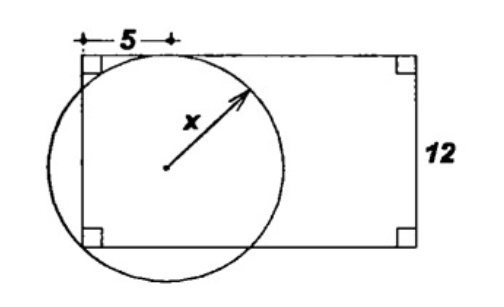
\includegraphics[width=6cm]{image1.geo}
         \end{figure}
         Hallar $x$.
      \end{section-problem}
   \end{frame}

   \begin{frame}
      \begin{section-problem}
         Si $P\left(x + \dfrac{1}{x}\right) = x^2 + \dfrac{1}{x^2} + 2023$, ¿cuál es el valor de $P(2024)$?
      \end{section-problem}
   \end{frame}

   \begin{frame}
      \begin{section-problem}
         Hallar $S$, si
         \[S = \left( \frac{1 + \dfrac{1}{3} - \dfrac{1}{2}}{2 - \dfrac{2}{3}} \right) \left( \frac{\dfrac{1}{2} + \dfrac{1}{3} + \dfrac{1}{6}}{\dfrac{1}{2} - \dfrac{2}{3} + \dfrac{3}{4}} \right)\]
      \end{section-problem}
   \end{frame}

   \begin{frame}
      \begin{section-problem}
         Indique el valor de la expresión
         \[E(3)  \cdot E(5) \cdot E(7) \cdots E(2021) \cdot E(2023)\]
         Si $E(x) = 1 + \dfrac{2}{x - 1}$
      \end{section-problem}
   \end{frame}

   \begin{frame}
      \begin{section-problem}
         En la figura se muestra un cuadrante, sobre el que se ha trazado la tangente $\overline{MN}$, de modo que $AM = 8$ y $BN = 9$.
         Hallar la medida de $R$
         \begin{figure}[htb]
            \centering
            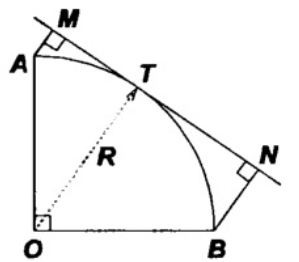
\includegraphics[width=5cm]{image4.geo}
         \end{figure}
      \end{section-problem}
   \end{frame}

   \begin{frame}
      \begin{section-problem}
         Hallar el resto de la división de
         \[
            \left[(x - 1)(x)(x + 2)(x + 3)\right]^2 + (x^2 + 2x)^3 x - 50
         \]
         entre $x^2 + 2x - 5$.
      \end{section-problem}
   \end{frame}

   \begin{frame}

      \begin{section-problem}
         Si $x^a y^b = 2^a$, $x^b y^a = 2^b$.
         Hallar el valor de $(xy)^{\dfrac{x}{y}}.$
      \end{section-problem}
   \end{frame}

   \begin{frame}
      \begin{section-problem}
         Si $P(x) = x^2 + 2x + 3$, calcule el valor de $P(1) + P(2) + \cdots + P(100).$
      \end{section-problem}
   \end{frame}

   \begin{frame}
      \begin{section-problem}
         ¿Cuántos triángulos se pueden contar, cómo máximo, en la siguiente figura?
         \begin{figure}[htb]
            \centering
            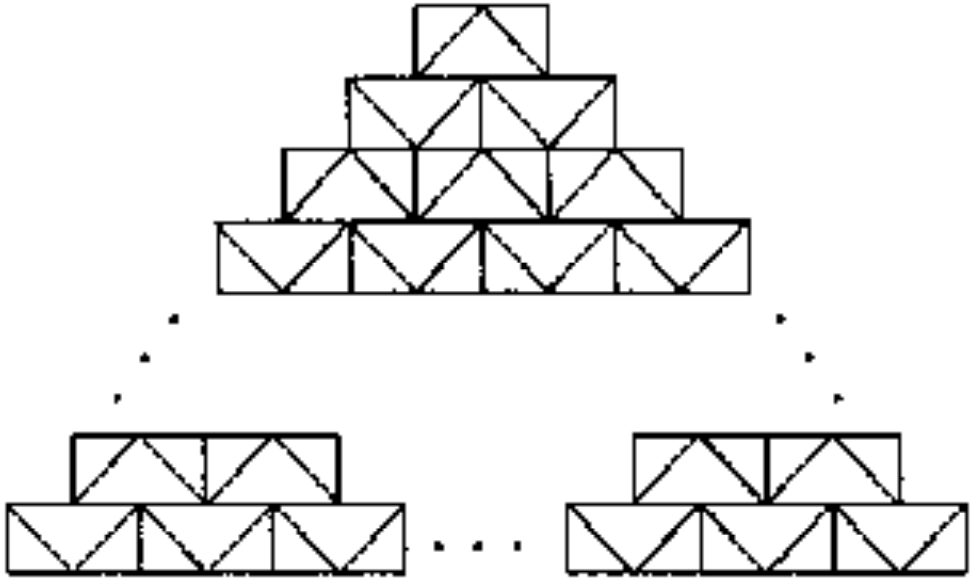
\includegraphics[width=4.5cm]{figura}
         \end{figure}
         Donde la base de esta figura tiene 2023 rectángulos.
      \end{section-problem}
   \end{frame}

   \begin{frame}
      \begin{section-problem}
         En la figura mostrada, calcular la medida de $OM$.
         \begin{figure}[htb]
            \centering
            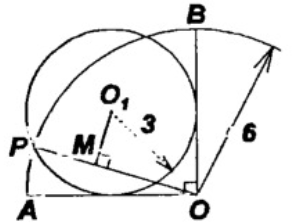
\includegraphics[width=5cm]{image2.geo}
         \end{figure}
      \end{section-problem}
   \end{frame}

   \begin{frame}
      \begin{section-problem}
         ¿Cuál es la suma de los factores de $P(x) = (x^2 + y^2 - 9)^2 - 4x^2 y^2$?
      \end{section-problem}
   \end{frame}

   \begin{frame}
      \begin{section-problem}
         La división de $987x^{17} - 1597x^{16} + 1$ por $x^2 - x + c$ genera el residuo $(a - b - 1)x^3 + (a + b - 7)x^2 + (a + c)x + b - d$, indique el valor de $(a - 3)^{2024} + (b - 4)^{2023} + 2022$.
      \end{section-problem}
   \end{frame}

   \begin{frame}
      \begin{section-problem}
         Un agricultor cosechó en el primer día $(x - 2)^{2023}$ granos de maíz y el segundo día $(x - 1)^{2024} + 7$ granos de maíz.
         Si el agricultor almacena los granos de los dos días en sacos, los cuales tiene una capacidad de $x^2 - 3x + 2$ granos cada uno.
         ¿cuál es el polinomio que representa los granos sobrantes?
      \end{section-problem}
   \end{frame}

   \begin{frame}
      \begin{section-problem}
         En la figura mostrada, hallar $\dfrac{AE}{AP}$.
         \begin{figure}[htb]
            \centering
            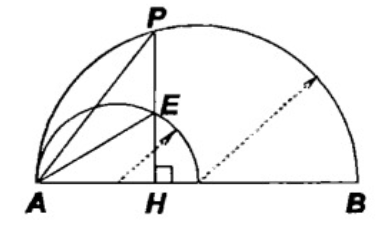
\includegraphics[width=5cm]{image3.geo}
         \end{figure}
      \end{section-problem}
   \end{frame}

   \begin{frame}
      \begin{section-problem}
         Cuál es el valor de $x$, si
         \[(1 + x) + (2 + x) + (3 + x) + \cdots + (n + x) = n^2 + 1012n\]
      \end{section-problem}
   \end{frame}
\end{document}